
%(BEGIN_QUESTION)
% Copyright 2006, Tony R. Kuphaldt, released under the Creative Commons Attribution License (v 1.0)
% This means you may do almost anything with this work of mine, so long as you give me proper credit

Identify which lamp in the following ladder-logic diagram is the {\it high-flow} alarm and which is the {\it low-flow} alarm, given the flow switch symbols shown:

$$\includegraphics[width=15.5cm]{i00548x01.eps}$$

\underbar{file i00548}
%(END_QUESTION)





%(BEGIN_ANSWER)

$$\includegraphics[width=15.5cm]{i00548x02.eps}$$

%(END_ANSWER)





%(BEGIN_NOTES)

Remember, the ``normal'' status of a switch is that state the switch is in when there is a {\it lack} of stimulus!  Therefore, a normally-closed flow switch will be closed when there is {\it no flow} going through it.

%INDEX% Measurement, flow: switch

%(END_NOTES)


